% F087｜牛顿切线法快速求近似根｜04_examples.tex
% 继承上传模板的 LaTeX 环境；当前条目的内容独立编写。
\clearpage
\begin{examplebox}
\textbf{\textcolor{CExample}{例 1：两次逼近根号 10}}
\par\medskip
\begin{center}
% F087｜steps 原创简明教学示意图
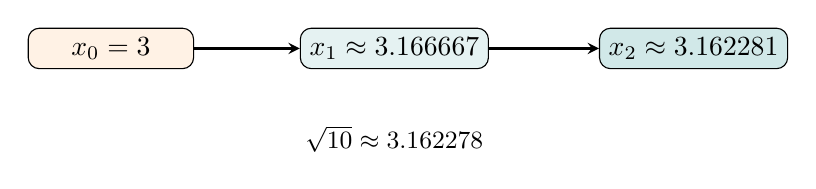
\begin{tikzpicture}[>=stealth,node distance=1cm]
\node[draw,rounded corners,fill=orange!10,minimum width=2.1cm] (a) at (0,0) {$x_0=3$};
\node[draw,rounded corners,fill=teal!10,minimum width=2.3cm] (b) at (3.6,0) {$x_1\approx3.166667$};
\node[draw,rounded corners,fill=teal!18,minimum width=2.3cm] (c) at (7.4,0) {$x_2\approx3.162281$};
\draw[->,thick] (a)--(b);\draw[->,thick] (b)--(c);
\node at (3.6,-1.15) {\small $\sqrt{10}\approx3.162278$};
\end{tikzpicture}

\end{center}
\medskip
取 $x_0=3$，\[x_1=\frac12\left(3+\frac{10}{3}\right)=\frac{19}{6}\approx3.166667.\]再算 $x_2=\dfrac12\left(\frac{19}{6}+\frac{60}{19}\right)=\frac{721}{228}\approx3.162281$；而 $\sqrt{10}\approx3.162278$。两步已很接近。
\end{examplebox}
\clearpage
\begin{examplebox}
\textbf{\textcolor{CExample}{例 2：估算立方根 71}}
\par\medskip
\begin{center}
% F087｜cube 原创简明教学示意图
\begin{tikzpicture}[>=stealth,scale=.88]
\node[draw,rounded corners,fill=teal!8,minimum width=8cm,minimum height=1.3cm] (a) at (4,0) {$x_{n+1}=\dfrac{2x_n+A/x_n^2}{3}$};
\node at (4,-1.0) {\small 三次根号也能用切线修正，不必背另一套思路};
\end{tikzpicture}

\end{center}
\medskip
$4^3=64<71<125=5^3$，取 $x_0=4$：\[x_1=\frac{2\cdot4+71/4^2}{3}=\frac{199}{48}\approx4.145833.\]代回立方后可知仍略偏大，再迭代一次约为 $4.140824$；真值约 $4.140818$。
\end{examplebox}
\clearpage
\begin{examplebox}
\textbf{\textcolor{CExample}{例 3：只比较大小，不需要迭代}}
\par\medskip
\begin{center}
% F087｜tangent 原创简明教学示意图
\begin{tikzpicture}[>=stealth,scale=.82]
\draw[->] (0,0)--(7.6,0) node[right]{$x$};\draw[->] (.8,-1.4)--(.8,3.2) node[above]{$y$};
% 横向比例尺 x_point=8(x-2.65)，纵向比例尺 y_point=0.75(x^2-10)。
\draw[teal,thick,domain=2.76:3.48,samples=45] plot ({8*(\x-2.65)},{.75*(\x*\x-10)});
% 在真实点 x_0=3 的切线；交轴位置 x_1=19/6。
\draw[orange,thick] (2,-1.2)--(6,1.05);
\fill[orange] (2.8,-.75) circle (2pt) node[below left=5pt]{$x_0=3$};
\fill[orange] (4.1333,0) circle(2pt) node[below=7pt]{$x_1\approx3.1667$};
\node at (5.5,2.7){\small 用切线寻找新的交点};
\node[teal] at (5.7,1.9){\small $y=x^2-10$};
\end{tikzpicture}

\end{center}
\medskip
判断 $\sqrt{10}>3.16$ 吗？直接验算 $3.16^2=9.9856<10$ 即可。\textbf{切线法适合求近似数值，不必每题都用。}
\end{examplebox}
